\section[Chương 5]{Chương 5: Cảm ứng điện từ}

\subsection{Câu 1}

Hiện tượng cảm ứng điện từ là hiện tượng hình thành một suất điện động trên vật dẫn khi vật dẫn được đặt trong một từ trường biến thiên.

Định luật Lenz: Dòng điện cảm ứng sinh ra có chiều sao cho từ trường do nó sinh ra có chiều chống lại nguyên nhân sinh ra nó.

\begin{itemize}
  \item Dịch chuyển 1 vòng dây kim loại trong từ trường để từ thông $\Phi_m$ thay đổi
  \item Trong thời gian $dt$, từ thông biến thiên một lượng $d\Phi_m$
  \item Xuất hiện dòng điện cảm ứng $I_c$
\end{itemize}

Khi đó công của từ lực lên dòng là $dA = I_cd\Phi_m$. Theo định luật Lenz thì công này là công cản (chống lại sự chuyển động). Để dây chuyển động ta cần công $dA'$

\begin{equation*}
  dA' = -dA = -I_cd\Phi_m
\end{equation*}

Công $dA'$ chuyển thành năng lượng của dòng cảm ứng

\begin{equation*}
  E_cI_cdt = -I_cd\Phi_m \Rightarrow E_c = -\frac{d\Phi_m}{dt}
\end{equation*}

Suất điện động cảm ứng bằng về trị số nhưng trái dấu với độ biến thiên của từ thông gửi qua diện tích của mạch.

\subsection{Câu 2}

\subsubsection{Hiện tượng tự cảm}

\begin{itemize}
  \item Ban đầu mạch đóng, điện kế chỉ vị trí $a$
  \item Nếu ngắt mạch thì kim điện kế chạy quá số $0$ rồi mới trở lại
  \item Nếu đóng mạch thì kin điện kế chạy quá $a$ rồi mới trở lại
\end{itemize}

Giải thích:

\begin{itemize}
  \item Khi ngắt mạch, $I$ về 0. Từ thông giảm, trong mạch xuất hiện dòng cảm ứng $I_c$ cùng chiều $I$ để chống lại sự giảm $\Rightarrow$ quá vạch
  \item Khi đóng mạch, $I$ tăng. Từ thông tăng, trong mạch xuất hiện dòng cảm ứng $I_c$ ngược chiều $I$ để chống lại sự tăng $\Rightarrow$ quá vạch
\end{itemize}

Nếu ta thay đổi $I$ trong mạch để từ thông do dòng đó gửi qua diện tích của mạch thay đổi thì trong mạch cũng xuất hiện dòng cảm ứng $I_c$. Vì dòng này do sự cảm ứng dòng trong mạch gây ra nên gọi là hiện tượng tự cảm.

Tính suất điện động tự cảm: Trong mạch đứng yên không đổi hình dạng, suất điện động tự cảm tỉ lệ và trái dấu với độ biến thiên cường độ dòng điện trong mạch.

\begin{equation*}
  E_{tc} = -L\frac{dI}{dt}
\end{equation*}

Xét cuộn dây thẳng dài 

\begin{gather*}
  B = \mu_0\mu \frac{n}{l}I \Rightarrow \Phi = nBS = \mu_0\mu \frac{n^2}{l} IS \\
  \Rightarrow L = \frac{\mu_0\mu n^2 S}{l}
\end{gather*}

\subsubsection{Hiệu ứng bề mặt}

Khi dòng điện cao tần chạy qua 1 dây dẫn thì do hiện tượng tự cảm, dòng điện đó hầu như không chạy trong lòng dây dẫn mà chỉ chạy ở mặt ngoài.

\newpage

\begin{figure*}[h]
  \centering
  \subfloat[\centering]{{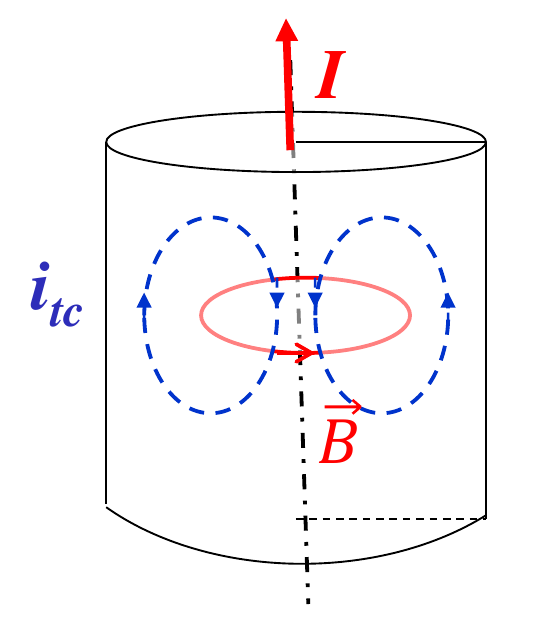
\includegraphics[width=0.3\textwidth]{ch05-1.png}}}
  \qquad
  \subfloat[\centering]{{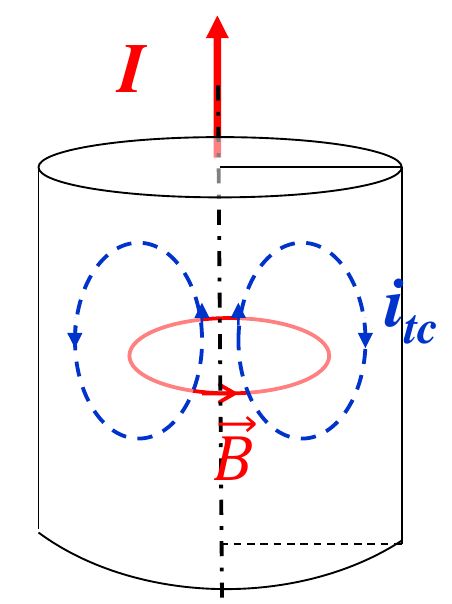
\includegraphics[width=0.3\textwidth]{ch05-2.png}}}
\end{figure*}

Giả sử dòng cao tần đi lên

\begin{itemize}
  \item Dòng $I$ sinh từ trường, biến thiên nên sinh $\vec{B}$ biến thiên
  \item Xét 1 tiết diện $S$ chứa trục đối xứng của dây, $\Phi_m$ qua đó biến thiên, sinh dòng tự cảm khép kín
\end{itemize}

Trong 1/4 chu kì đầu, giả sử dòng đang tăng

\begin{itemize}
  \item $\Phi_m$ qua $S$ tăng, $I_{tc}$ sỉnh $\vec{B}'$ chống lại $\vec{B}$, dòng có chiều như hình (a).
  \item Bên trong thì $I_{tc}$ ngược chiều $I$, dòng giảm
  \item Trên bề mặt $I_{tc}$ cùng chiều $I$, dòng tăng 
\end{itemize}

Trong 1/4 chu kì sau, dòng đang giảm

\begin{itemize}
  \item $\Phi_m$ qua $S$ giảm, $I_{tc}$ sinh $\vec{B}'$ chống lại $\vec{B}$, dòng có chiều như hình (b).
  \item Bên trong thì $I_{tc}$ cùng chiều $I$, dòng mạnh lên
  \item Trên bề mặt $I_{tc}$ ngược chiều $I$, dòng giảm đi
\end{itemize}

Ứng dụng:

\begin{itemize}
  \item Tôi kim loại ở bề mặt
  \item Làm dây dẫn rỗng để tiết kiệm kim loại
\end{itemize}

\subsection{Câu 3}

Áp dụng định lý Ôm trong mạch 

\begin{gather*}
  E + E_{tc} = IR \Rightarrow E = IR + L\frac{dI}{dt} \\
  EIdt = RI^2dt + LIdI
\end{gather*}

Vậy trong quá trình thành lập dòng thì phần năng lượng của nguồn tiềm tàng dưới dạng năng lượng từ trường là

\begin{equation*}
  W_m = \int_{0}^{W_m} dW_m = \int_{0}^{I} LIdI = \frac{1}{2}LI^2
\end{equation*}

Mật độ năng lượng từ trường:

\begin{equation*}
  w_m = \frac{W_m}{V} = \frac{\frac{1}{2}LI^2}{V} = \frac{1}{2} \frac{\mu_0\mu n^2 SI^2}{l^2 S} = \frac{1}{2} \mu_0 \mu \frac{n^2}{l^2} I^2
\end{equation*}

Có $B = \mu_0\mu \frac{n}{l} I$

\begin{equation*}
  w_m = \frac{1}{2} BH
\end{equation*}

Năng lượng từ trường bất kỳ:

\begin{equation*}
  W_m = \int_V w_mdV = \frac{1}{2} \int_V BHdV
\end{equation*}